%!TEX program = xelatex
\documentclass[aspectratio=169]{beamer}
\usepackage{lmodern}
\usefonttheme[onlymath]{serif}
\usepackage{blindtext}
\usepackage{booktabs} % for professional tables
\usepackage{bm}
\usepackage{minted}
\usepackage{amsmath, amssymb}
\usepackage{tikzsymbols}
\usepackage{smartdiagram}
\usepackage{subcaption}
\usepackage{fontawesome}
\usepackage{listings}
\usepackage{xcolor}

\definecolor{codegreen}{rgb}{0,0.6,0}
\definecolor{codegray}{rgb}{0.5,0.5,0.5}
\definecolor{codepurple}{rgb}{0.58,0,0.82}
\definecolor{backcolour}{rgb}{0.95,0.95,0.92}

%\lstdefinestyle{mystyle}{
%    backgroundcolor=\color{backcolour},
%    commentstyle=\color{codegreen},
%    keywordstyle=\color{magenta},
%    numberstyle=\tiny\color{codegray},
%    stringstyle=\color{codepurple},
%    basicstyle=\ttfamily\footnotesize,
%    breakatwhitespace=false,
%    breaklines=true,
%    captionpos=b,
%    keepspaces=true,
%    numbers=left,
%    numbersep=5pt,
%    showspaces=false,
%    showstringspaces=false,
%    showtabs=false,
%    tabsize=2,
%}
%
%\lstset{style=mystyle,
%        otherkeywords={!,!=,~,$,*,\&,\%/\%,\%*\%,\%\%,<-,<<-}
%}
\lstset{
    language=R,
    basicstyle=\ttfamily,
    keywordstyle=\color{red}\bfseries,
    otherkeywords={!,!=,~,$,*,\&,\%/\%,\%*\%,\%\%,<-,<<-},
    escapeinside=||,
}

\usepackage[linesnumbered,ruled,vlined]{algorithm2e}
\newcommand\blfootnote[1]{%
  \begingroup
  \renewcommand\thefootnote{}\footnote{#1}%
  \addtocounter{footnote}{-1}%
  \endgroup
}

% convenient notations
\newcommand{\bT}{\boldsymbol{\Theta}}
\newcommand{\tr}{\mathsf{tr}}
\newcommand{\zero}{\bm{0}}
\newcommand{\one}{\bm{1}}
\newcommand{\lmd}{\boldsymbol{\lambda}}
\newcommand{\bgamma}{\boldsymbol{\gamma}}
\newcommand{\Diag}{\mathsf{Diag}}
\newcommand{\XX}{\mathbb{X}}
\newcommand{\ba}{\bm{a}}
\newcommand{\uu}{\bm{u}}
\newcommand{\zz}{\bm{z}}
\newcommand{\ww}{\bm{w}}
\newcommand{\WW}{\bm{W}}
\newcommand{\qq}{\bm{q}}
\newcommand{\QQ}{\bm{Q}}
\newcommand{\KK}{\bm{K}}
\newcommand{\UU}{\bm{U}}
\newcommand{\JJ}{\bm{J}}
\newcommand{\II}{\bm{I}}
\newcommand{\bS}{\bm{S}}
\newcommand{\bY}{\bm{Y}}
\newcommand{\bX}{\bm{X}}
\newcommand{\RR}{\mathbb{R}}
\newcommand{\EE}{\mathbb{E}}
\newcommand{\PP}{\mathbb{P}}
\newcommand{\sL}{\mathcal{L}}
\newcommand{\sA}{\mathcal{A}}
\newcommand{\sD}{\mathfrak{d}}
\newcommand{\sX}{\mathcal{X}}
\newcommand{\sY}{\mathcal{Y}}
\DeclareMathOperator*{\argmin}{arg\,min}
\DeclareMathOperator*{\argmax}{arg\,max}
\DeclareMathOperator*{\supp}{supp}
\def\vec#1{{\ensuremath{\bm{{#1}}}}}
\def\mat#1{\vec{#1}}
\newcommand{\norm}[1]{\left\lVert#1\right\rVert}

\usetheme{Execushares}

\title{Industry Classification Using Graphs}
\subtitle{\large{Fifteenth Annual R/Finance Conference, Chicago, USA}}
\author{\normalsize{\textbf{Vin\'icius Cardoso}}}
\date{May, 2023}

\setcounter{showSlideNumbers}{1}

\begin{document}
  \setcounter{showProgressBar}{0}
  \setcounter{showSlideNumbers}{0}

  \frame{\titlepage}

  %      \begin{frame}
  %        \frametitle{Contents}
  %            \vspace{.5cm}
  %        \begin{enumerate}
  %          \item Introduction \& Background
  %           \\ \textcolor{ExecusharesGrey}{\footnotesize\hspace{1em} graphs and heavy-tails in financial markets}
  %          \item Proposed Algorithms
  %           \\ \textcolor{ExecusharesGrey}{\footnotesize\hspace{1em} student-t formulation and the alternating direction method of multipliers}
  %           \item Applications
  %           \\ \textcolor{ExecusharesGrey}{\footnotesize\hspace{1em} clustering financial time-series}
  %           \item Conclusions
  %        \end{enumerate}
  %      \end{frame}

  \setcounter{showSlideNumbers}{0}
  \setcounter{framenumber}{0}
  \setcounter{showProgressBar}{1}
  \setcounter{showSlideNumbers}{1}

 \begin{frame}{Team}
  \vspace{1cm}
   \begin{figure}
       \captionsetup[subfigure]{justification=centering}
       \centering
       \begin{subfigure}[t]{0.3\textwidth}
           \centering
       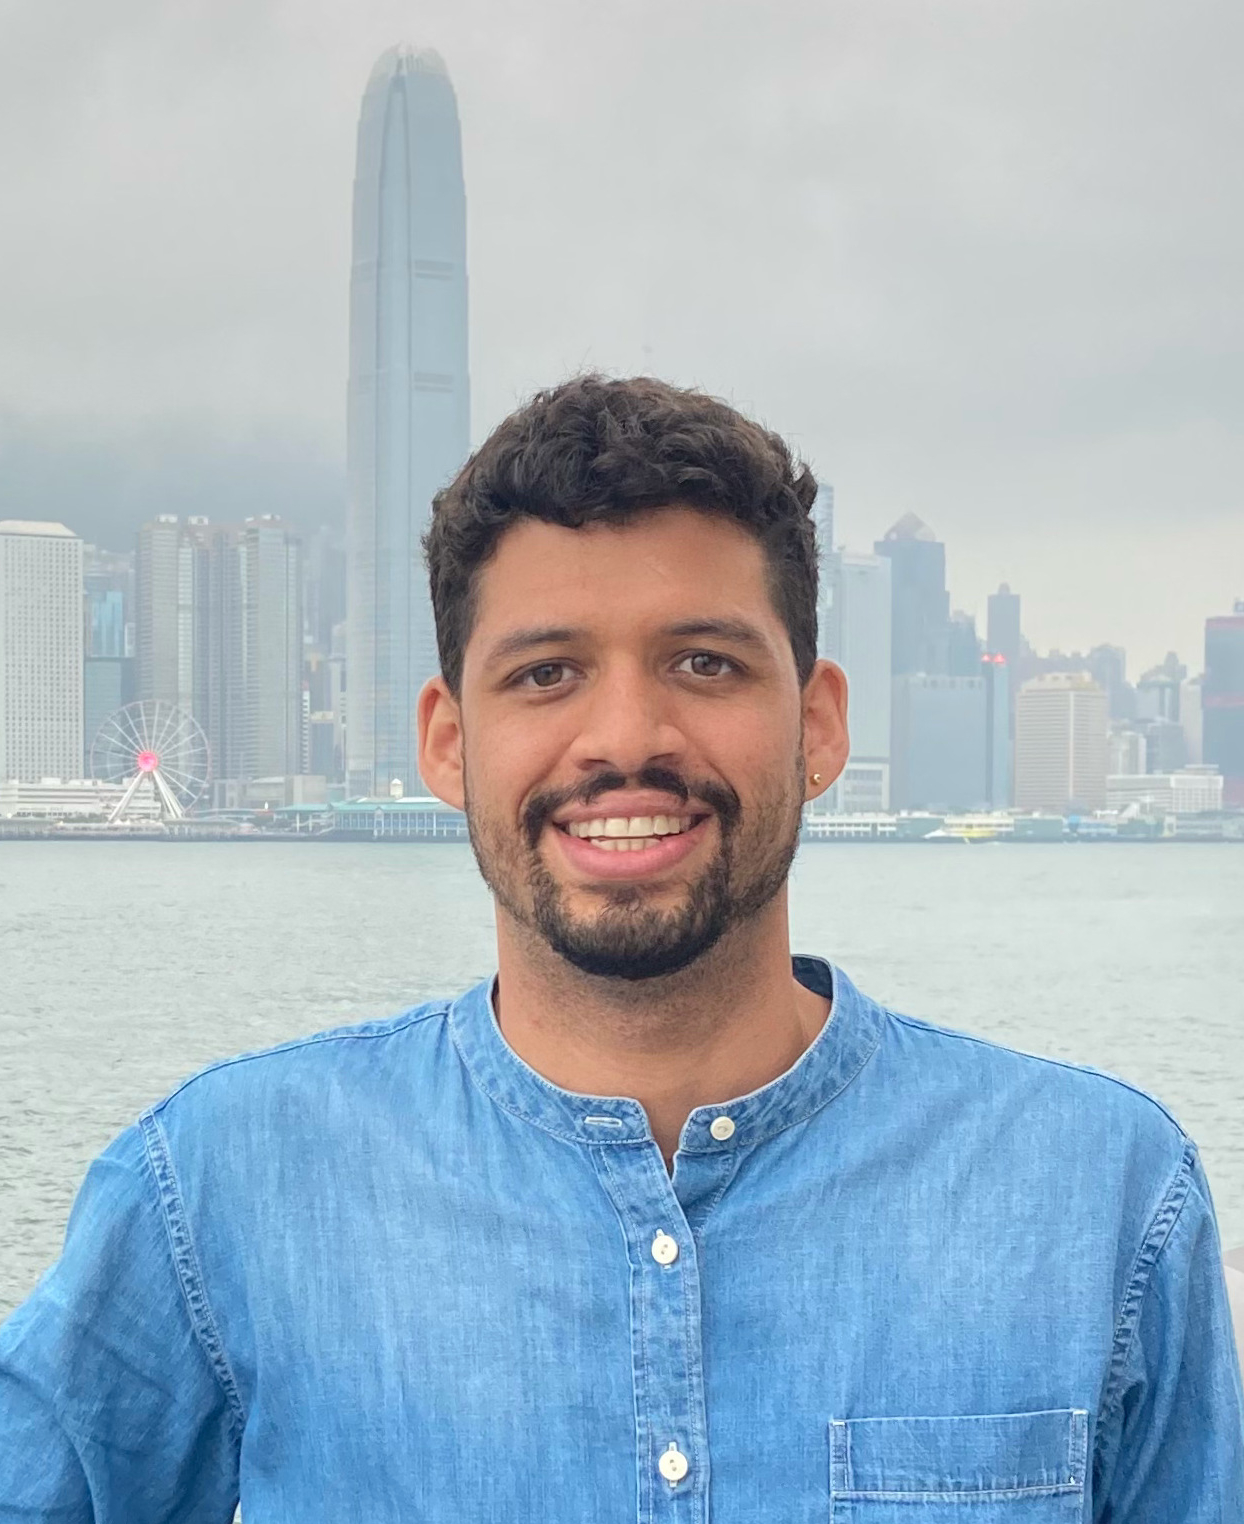
\includegraphics[scale=.093]{profile.jpg}
       \end{subfigure}%
       ~~~
   \begin{subfigure}[t]{0.3\textwidth}
       \centering
           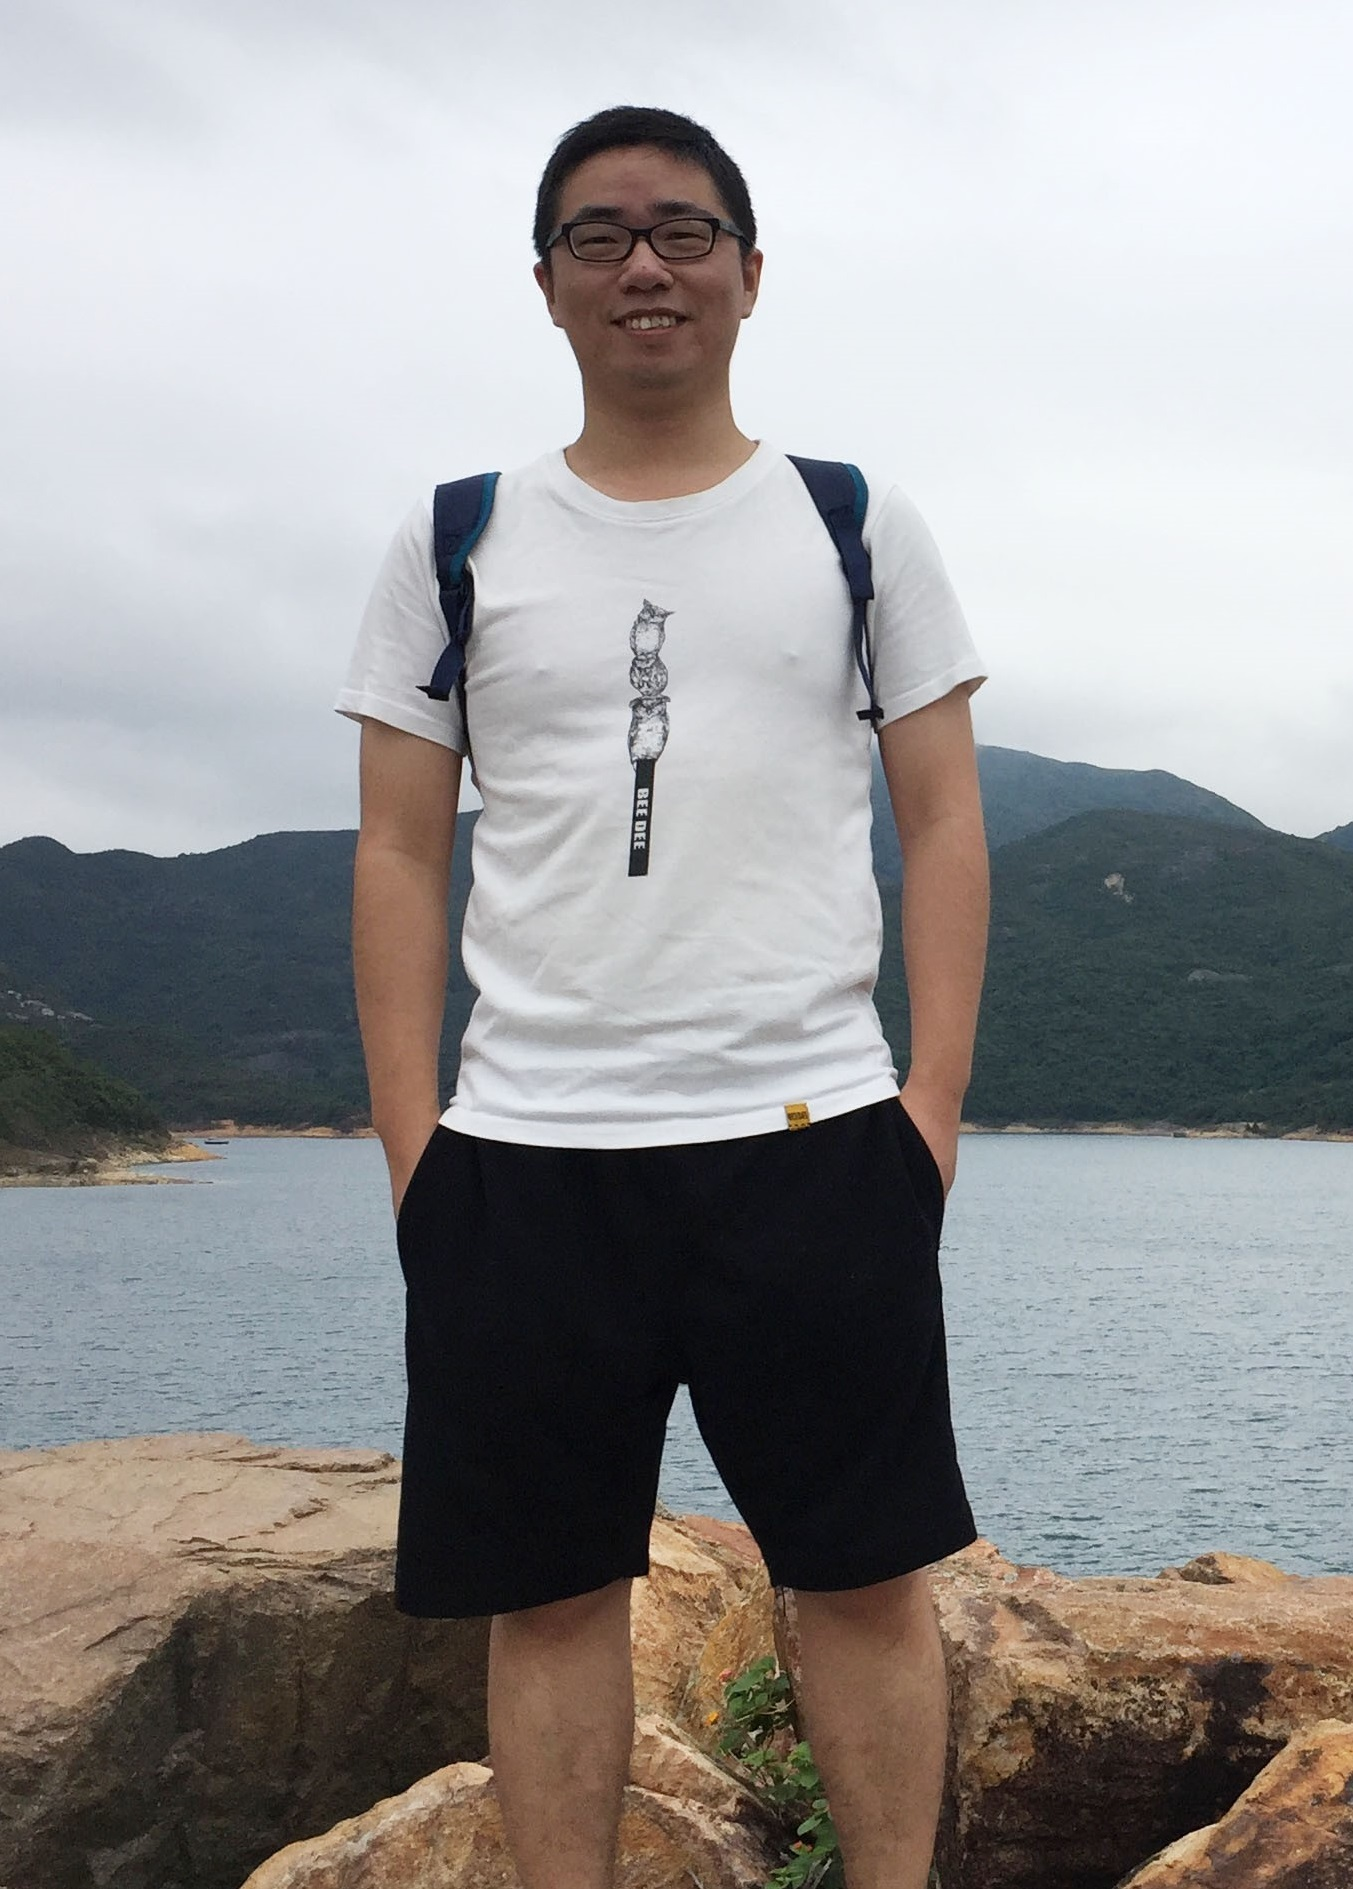
\includegraphics[scale=.076]{photo-jiaxi.jpg}
   \end{subfigure}
   ~~~
   \begin{subfigure}[t]{0.3\textwidth}
       \centering
           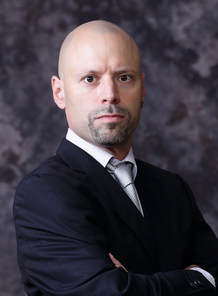
\includegraphics[scale=.48]{photo-daniel.jpg}
   \end{subfigure}
   \end{figure}
\end{frame}

\begin{frame}{Gist}
\begin{minipage}[0.2\textheight]{\textwidth}
  \begin{columns}[T]
  \begin{column}{0.5\textwidth}
       \begin{center}
          \smartdiagram[circular diagram:clockwise]{
              Financial Data,
              Graphs (Models),
              Optimize,
              Visualize}
       \end{center}
  \end{column}
  \begin{column}{0.5\textwidth}
    \vspace{1.5cm}
    \pause
    \begin{itemize}
      \item Key ideas:
   \begin{itemize}
    \pause
   \item \textbf{model} a financial networks as undirected graph
   \pause
   \item \textbf{use} such graphs as a \textbf{tool} for industry \textbf{classification} of stocks or \textbf{clustering} cryptocurrencies
   \end{itemize}
  \end{itemize}
  \end{column}
  \end{columns}
  \end{minipage}
\end{frame}
%
\begin{frame}{Motivation and Goals}
  \vspace{1cm}
  \begin{itemize}
    \pause
    \item financial \textbf{stocks} are often \textbf{grouped} together: industry, market area, portfolio diversification etc
    \pause
    \item standard for stock \textbf{industry} \textbf{classification}: Global Industry Classification Standard (GICS)\footnote{\url{https://www.msci.com/our-solutions/indexes/gics}}
    \pause
    \item we provide \textbf{tools} for anyone to create their own, \textbf{bespoke classification} system 
    \pause
    \item result of our research efforts:
    \begin{itemize}
      \item \textbf{NeurIPS'22} Cardoso, J. V. M., Ying, J., and Palomar, D. P. ``Learning Bipartite Graphs: Heavy Tails and Multiple Components'',
      \textit{Advances in Neural Information Processing Systems}, 14044--14057 (35), 2022
      \item \textbf{NeurIPS'21} Cardoso, J. V. M., Ying, J., and Palomar, D. P. ``Graphical Models in Heavy-Tailed Markets'',
      \textit{Advances in Neural Information Processing Systems}, 19989--20001 (34), 2021 
    \end{itemize}
  \end{itemize}
\end{frame}

\begin{frame}{Light Primer on Graphs}
    \pause
  \vspace{1cm}
  \begin{figure}
       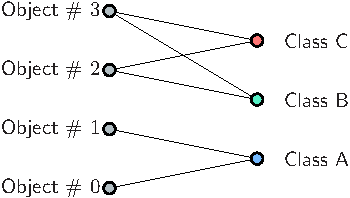
\includegraphics[scale=1.5]{figures/k-comp-bipartite-crop.pdf}
  \end{figure}
\end{frame}
\begin{frame}{Light Primer on Graphs}
  \vspace{1cm}
  \begin{figure}
       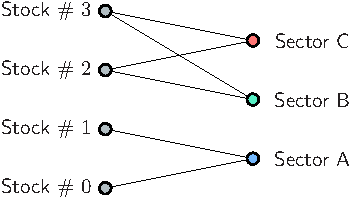
\includegraphics[scale=1.5]{figures/k-comp-bipartite-crop-finance.pdf}
  \end{figure}
  \pause
  \begin{itemize}
    \item hierarchical classification
  \end{itemize}
\end{frame}
\section*{goal: estimate the edges that connect stocks to sectors}

\begin{frame}{Graph Estimation}
  \begin{itemize}
    \pause
    \item graphs are matrices: Laplacian matrix $\bm{L}$ of a graph \textbf{encodes} the \textbf{edge weights}
    \pause
    \item given a matrix of \textbf{stock features} $\bm{X} \in \mathbb{R}^{n\times p}$
    \pause
    \item \`a la Graphical Lasso (Sparse Inverse Covariance Matrix estimation):
  \end{itemize}
  \begin{center}
    \begin{tabular}{@{}l@{}}
        \large
        $
    \begin{array}{cl}
      \underset{\bm{L} \succeq \mathbf{0}}{\mathsf{minimize}} & \frac{1}{n}\mathsf{tr}\left(\bm{X}\bm{L}\bm{X}^\top\right)
      - \log\mathrm{det}^{*}\left(\bm{L}\right),\\
      \mathsf{subject~to} & \bm{L}\mathbf{1} = \mathbf{0},~L_{ij} = L_{ji} \leq 0, \bm{L} \in \mathfrak{L}
    \end{array}
        $
    \end{tabular}
\end{center}
\pause
\begin{itemize}
  \item \textbf{R packages}
\end{itemize}
\begin{itemize}
  \item[] 
\includegraphics[scale=.1]{figures/github.png} \url{https://github.com/convexfi/fingraph}
  \item[] 
\includegraphics[scale=.1]{figures/github.png} \url{https://github.com/convexfi/bipartite}
\end{itemize}
    %\begin{center}
    %    \begin{tabular}{@{}l@{}}
    %      \huge$\mathcal{G} = \left(\mathcal{V}, \mathcal{E}, \bm{W}\right)$
    %    \end{tabular}
    %  \end{center}
    %\begin{itemize}
    %    \item \Large$\mathcal{V} =  \left\{1, 2, \dots, p\right\}$
    %    \item $\mathcal{E} \displaystyle \subseteq \left\{\left\{u, v\right\}: u,v \in \mathcal{V}, u \neq v\right\}$
    %    \item {\bf Adjacency Matrix:} $\bm{W} \in \mathbb{R}_{+}^{p\times p}, \bm{W} = \bm{W}^\top, \mathsf{diag}(\bm{W}) = \mathbf{0}$
    %    \item {\bf Degree Matrix:} $\bm{D} = \mathsf{Diag}(\bm{W}\mathbf{1})$
    %    \item {\bf Laplacian Matrix:} $\bm{L} = \bm{D} - \bm{W}$
    %\end{itemize}
\end{frame}

\begin{frame}{Stock Industry Classification}
  \pause
  \vspace{.75cm}
  \begin{figure}[!htb]
  \captionsetup[subfigure]{justification=centering}
  \centering
  \begin{subfigure}[t]{0.99\textwidth}
      \centering
      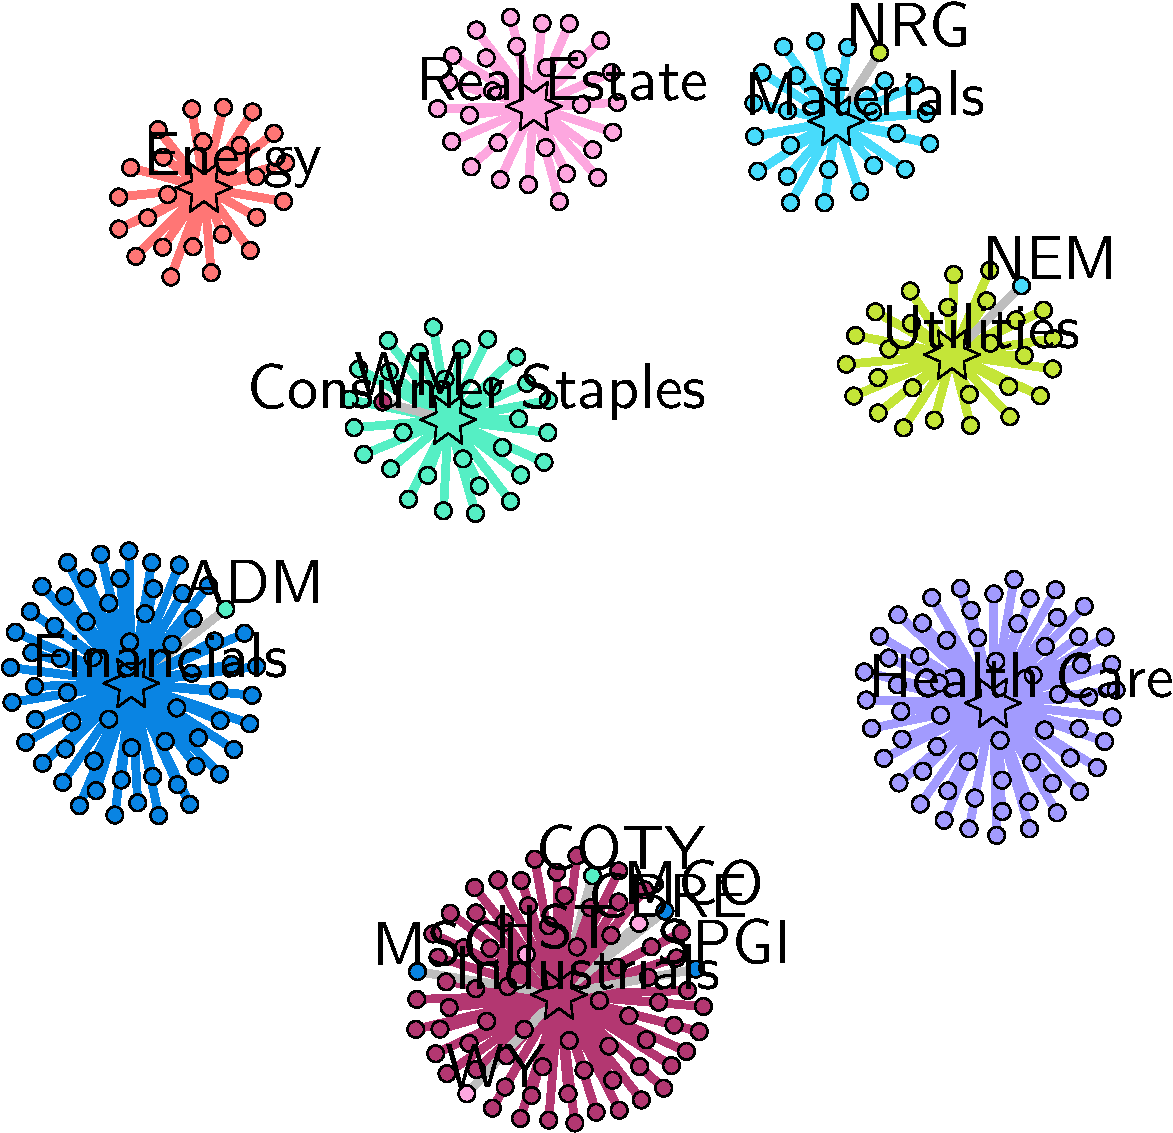
\includegraphics[scale=0.38]{figures/bipartite-heavy-tail-kcomp-labels-crop.pdf}
  \end{subfigure}%
 \end{figure}
\end{frame}

\begin{frame}{Clustering Cryptocurrencies}
  \pause
    \vspace{.75cm}
    \begin{figure}[!htb]
    \captionsetup[subfigure]{justification=centering}
    \centering
    \begin{subfigure}[t]{0.99\textwidth}
        \centering
        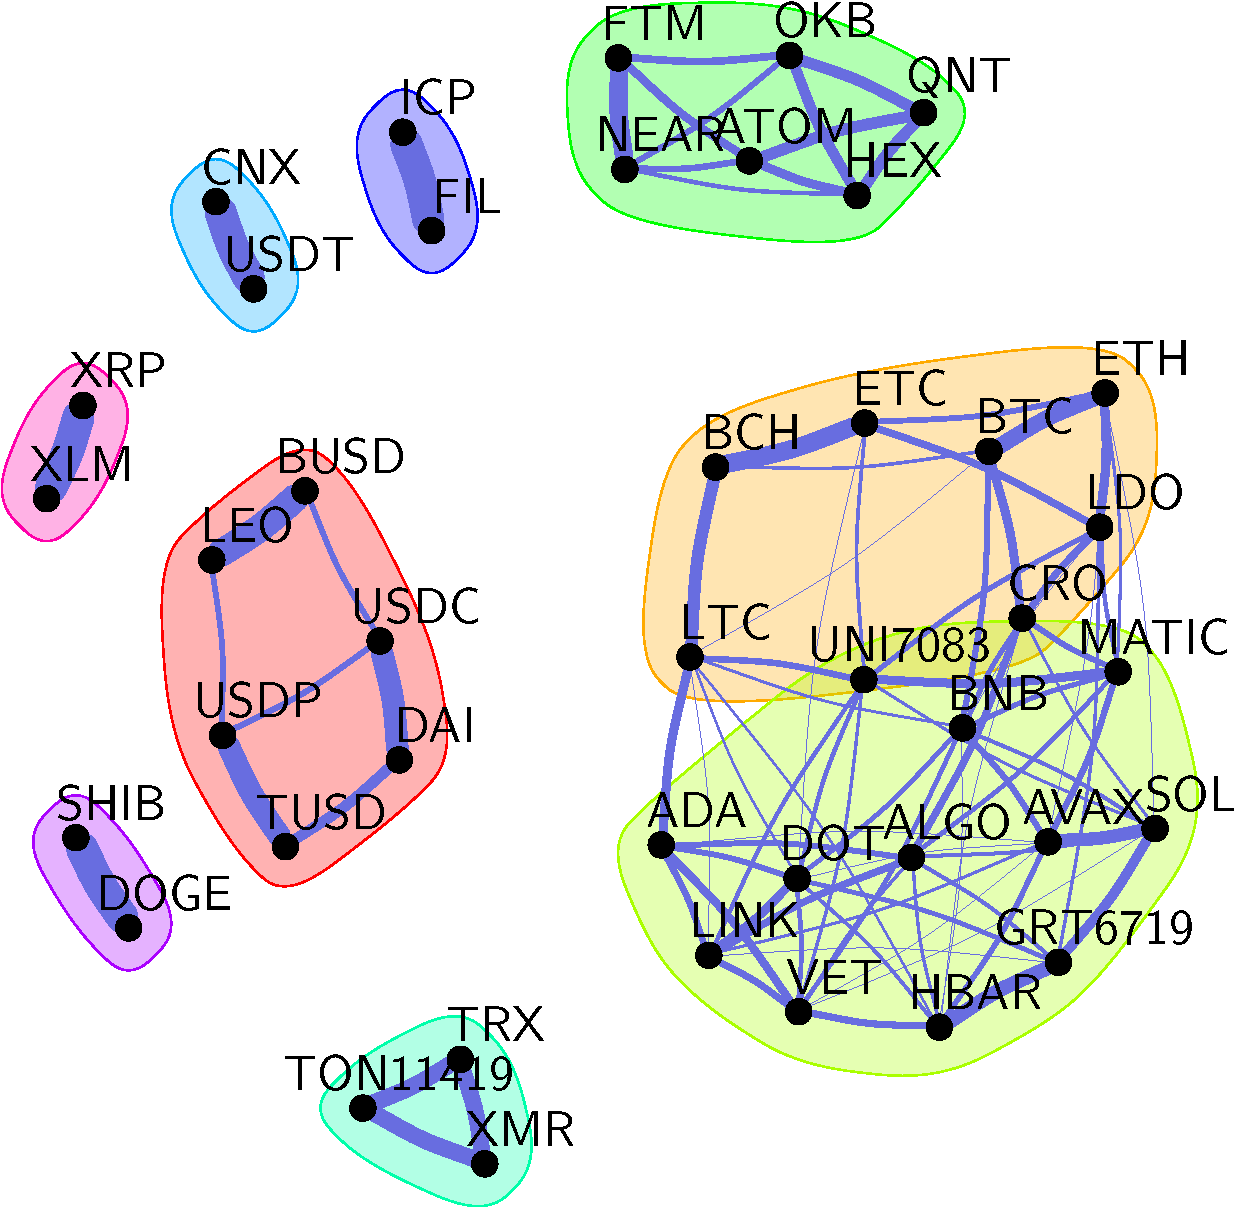
\includegraphics[scale=0.38]{figures/crypto-45-crop.pdf}
    \end{subfigure}%
   \end{figure}
\end{frame}

\begin{frame}[fragile]
\frametitle{R Pseudocode}
\begin{lstlisting}[language=R]
library(xts)
library(quantmod)
library(igraph)
library(fingraph)

stock|\_|features <- query|\_|features(...)
stock|\_|graph <- estimate|\_|graph(stock|\_|features,
                             hyperparameters=...)
plot(stock|\_|graph)
\end{lstlisting}
\end{frame}

\begin{frame}{Thank You!!}
  \begin{itemize}
    \item {\Large\faicon{envelope}} \url{jvdmc@connect.ust.hk}
    \item {\Large \faicon{github}} \url{https://github.com/convexfi}
    \item {\Large \faicon{firefox}} \url{https://mirca.github.io}
    \item {\Large \faicon{twitter}} \url{@mircaze}
  \end{itemize}
\end{frame}

\end{document}
